32. $\cfrac{x^2}{x+2}\leqslant -x\Leftrightarrow\cfrac{x^2+x^2+2x}{x+2}\leqslant 0\Leftrightarrow\cfrac{2x(x+1)}{x+2}\leqslant 0.$
Применив метод интервалов, найдём ответ:
\begin{figure}[ht!]
\center{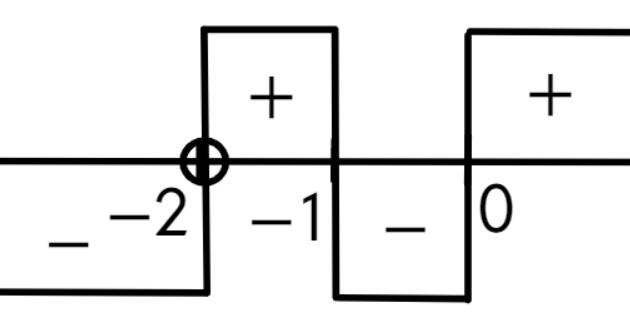
\includegraphics[scale=0.35]{int32.png}}
\end{figure}
$x\in(-\infty;-2)\cup[-1;0].$\\
